\subsection{Lab14: Transmisión de señales de radio FM para Walkie-Talkie UHF}

%*********************
\begin{frame}{}

\pgfdeclareimage[width=\paperwidth,height=\paperheight]{bg}{imagenes/fondo_lab}
\setbeamertemplate{background}{\pgfuseimage{bg}}

\bfseries{\textrm{\LARGE Lab14 \newline \Large Transmisión de señales de\newline radio FM para Walkie-Talkie \newline UHF 
}}
\raggedright
\end{frame}
%*********************


\begin{frame}{Transmisión FM para Walkie-Talkie UHF}

\pgfdeclareimage[width=\paperwidth,height=\paperheight]{bg}{imagenes/fondo3}
\setbeamertemplate{background}{\pgfuseimage{bg}}

Para este laboratorio se utilizará radio definida por software, con el fin de realizar la transmisión de las señales de radiofrecuencia modulada en la banda de UHF en donde se encuentran las frecuencias de cada uno de los canales del dispositivo Motorola EP150, el cual será utilizado para llevar acabo correctamente la práctica.
\end{frame}
%---------------------------------

\begin{frame}{Diagrama general}

\begin{figure}[H]
\centering
\vspace{-1mm}
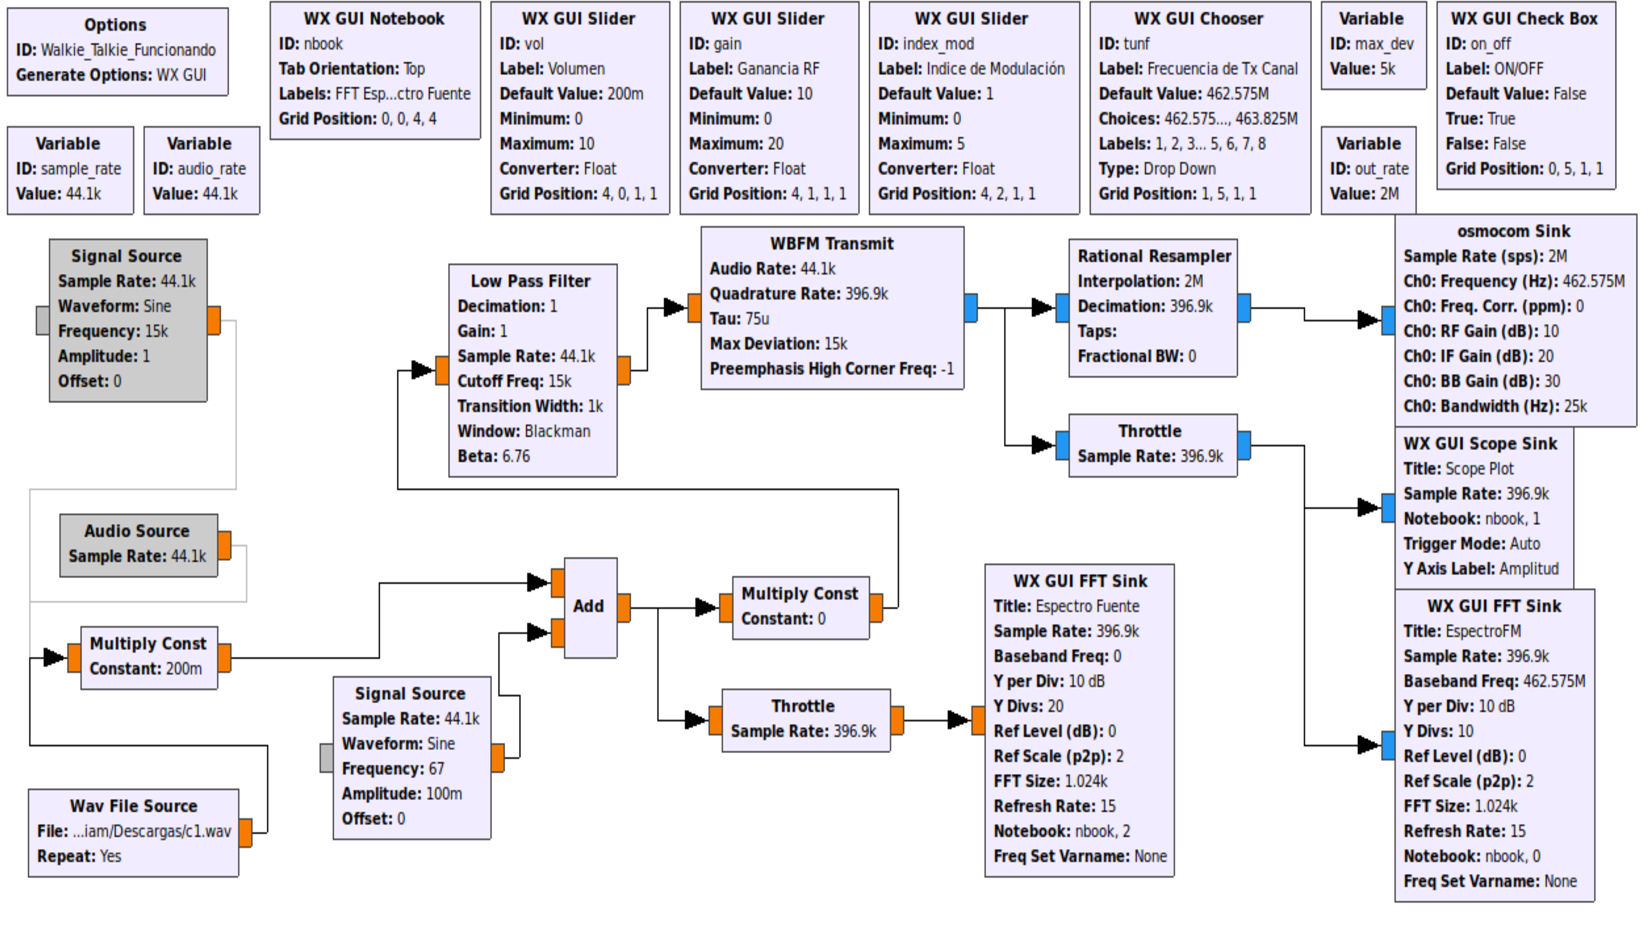
\includegraphics[width=\textwidth]{parte3/lab14/pdf/Lab14_2.pdf}
\end{figure}

\end{frame}
%---------------------------------

\begin{frame}{Tonos privados}

\textbf{CTCSS}\\
\vspace{3mm}
El sistema continuo de silenciamiento codificado por tonos o CTCSS es un circuito que se utiliza para reducir la molestia de escuchar a otros usuarios en un canal compartido de comunicaciones de radio bidireccionales. A veces se lo conoce como silenciamiento de tono. Lo hace agregando un tono de audio de baja frecuencia a la voz. Cuando más de un grupo de usuarios está en la misma frecuencia de radio (llamados usuarios co-canal), los circuitos CTCSS silencian a los usuarios que están utilizando un tono CTCSS diferente o no CTCSS \cite{Wikipedia2018}.
\end{frame}
%---------------------------------

\begin{frame}{Detección de portadoras y tonos privados}

Para este procedimiento es necesario contar con el software SDR-Sharp el cual es un analizador de espectro de frecuencias y además cuenta con la función de detector de tonos privados CTCSS (actualmente solo cuenta con soporte para Windows), sumado a esto también se utilizará el dispositivo HackRF-One como receptor de señales FM, además del transmisor Motorola EP150 \cite{Airspy2018}.

\end{frame}
%---------------------------------

\begin{frame}{Detección de portadoras y tonos privados}

\begin{figure}[H]
\centering
\vspace{-3mm}
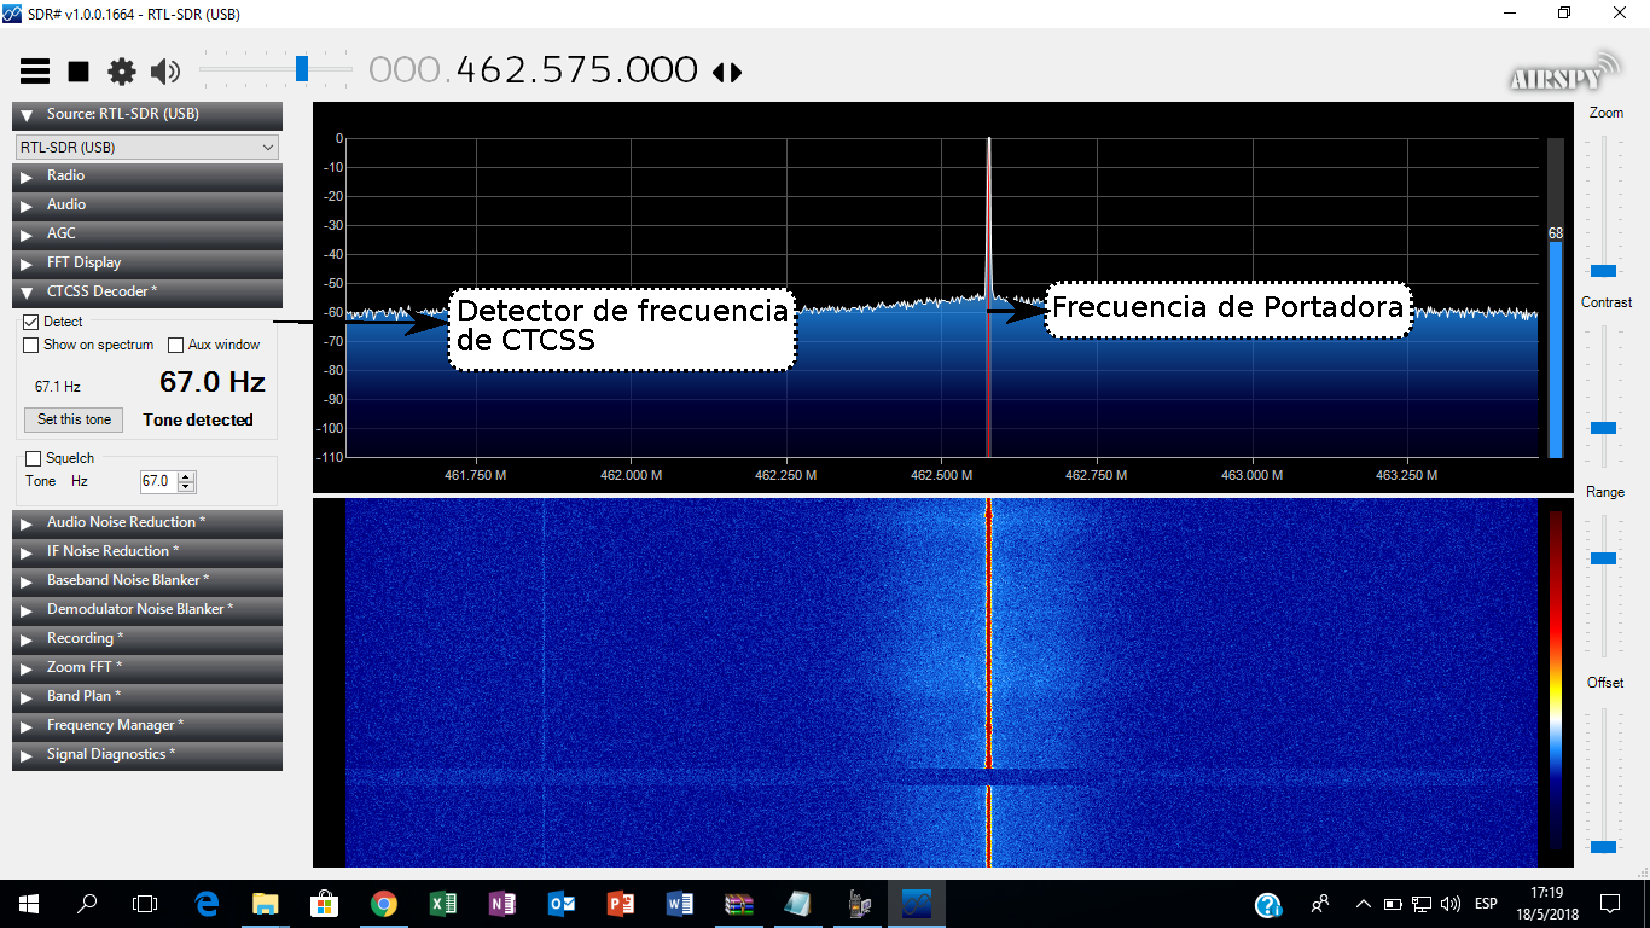
\includegraphics[width=0.9\textwidth]{parte3/lab14/pdf/Lab14_1.pdf}
\end{figure}

\end{frame}
%---------------------------------

\begin{frame}{Frecuencias de la señal de portadora}

Como se mostró en la figura anterior se pueden observar la frecuencia de las portadoras de cada canal y su respectivo tono CTCSS el cual es 67 Hz como se muestra en la siguiente tabla, dado el caso de que las portadoras halladas y sus tonos no correspondan con la tabla es necesario reiniciar el dispositivo a sus valores de fábrica véase el manual \cite{Motorola2010}.


\begin{table}[]
\scriptsize
\centering
\begin{tabular}{|c|c|}
\hline

\rowcolor{BlueGreen!20}
\textbf{CANAL} & \textbf{FRECUENCIA DE SEÑAL PORTADORA} \\ \hline
1              & 462,5750 MHz                           \\ \hline
2              & 462,6250 MHz                           \\ \hline
3              & 462,6750 MHz                           \\ \hline
4              & 463,5500 MHz                           \\ \hline
5              & 463,6250 MHz                           \\ \hline
6              & 463,7625 MHz                           \\ \hline
7              & 463,7750 MHz                           \\ \hline
8              & 463,8250 MHz                           \\ \hline
\end{tabular}
\end{table}

\end{frame}
%---------------------------------

\begin{frame}{Desarrollo del diagrama en GNU Radio}

Las variables necesarias para el desarrollo del esquema son:
\begin{itemize}
    \item {\textit{sample\_rate} = Frecuencia de muestreo general}
    \item {\textit{audio\_rate} = Frecuencia de muestreo del audio (se suele utilizar 44.1KHz)}
    \item {\textit{out\_rate} = Frecuencia de muestreo del dispositivo HackRF-One}
    \item {\textit{max\_dev} = Desviación máxima en frecuencia de la señal modulada (viene dada por el producto index\_mod*15KHz el cual es el estándar para WBFM)}
    
\end{itemize}{}

\end{frame}
%---------------------------------

\begin{frame}{Desarrollo del diagrama en GNU Radio}

También es necesario utilizar un grupo de slider entre los que encontramos:
\begin{itemize}
    \item {\textit{vol}  = Volumen del audio}
    \item {\textit{index\_mod} = Índice de modulación (suele utilizarse un índice entre 1 y 5)}
    \item {\textit{gain} = Ganancia RF (ganancia prevista por parte de la tarjeta)}
    \item {\textit{tunf} = Frecuencia de Tx (frecuencia de las distintas portadoras de los canales)}
    
\end{itemize}{}

\end{frame}
%---------------------------------

\begin{frame}{Desarrollo del diagrama en GNU Radio}

Para comenzar con el diagrama de transmisiones es necesario incluir el audio que se desea transmitir esto se puede lograr cargando un archivo WAV (bloque WAV file source), mediante el micrófono del equipo (bloque Audio Source) o finalmente a partir de un generador de señales (bloque Signal Source) seguido a esto se multiplica por una constante, cuyo valor esta dado por el slider vol, con el fin de obtener la amplitud deseada, dicha amplitud no debe exceder los 200m, como se observa a continuación:

\begin{figure}[H]
\centering
\vspace{-3mm}
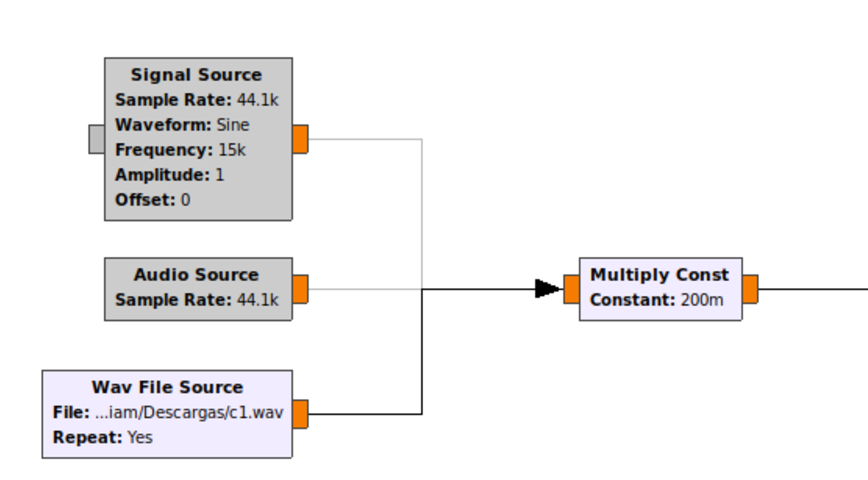
\includegraphics[width=0.7\textwidth]{parte3/lab14/pdf/Lab14_3.pdf}
\end{figure}


\end{frame}
%---------------------------------

\begin{frame}{Desarrollo del diagrama en GNU Radio}

Luego se añade el tono CTCSS a la información a transmitir esto con el fin de que la señal transmitida pueda ser escuchada desde el dispositivo Walkie-Talkie como se puede observar:

\begin{figure}[H]
\centering
\vspace{-3mm}
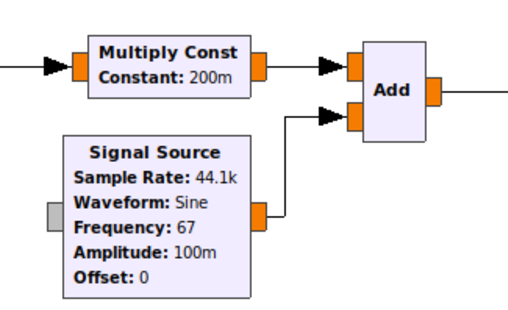
\includegraphics[width=0.6\textwidth]{parte3/lab14/pdf/Lab14_4.pdf}
\end{figure}

\end{frame}
%---------------------------------

\begin{frame}{Desarrollo del diagrama en GNU Radio}

En la siguiente etapa se implementa un filtro pasa bajas a la señal evitando frecuencias altas que puedan agregar ruido durante la transmisión.

\begin{figure}[H]
\centering
\vspace{-3mm}
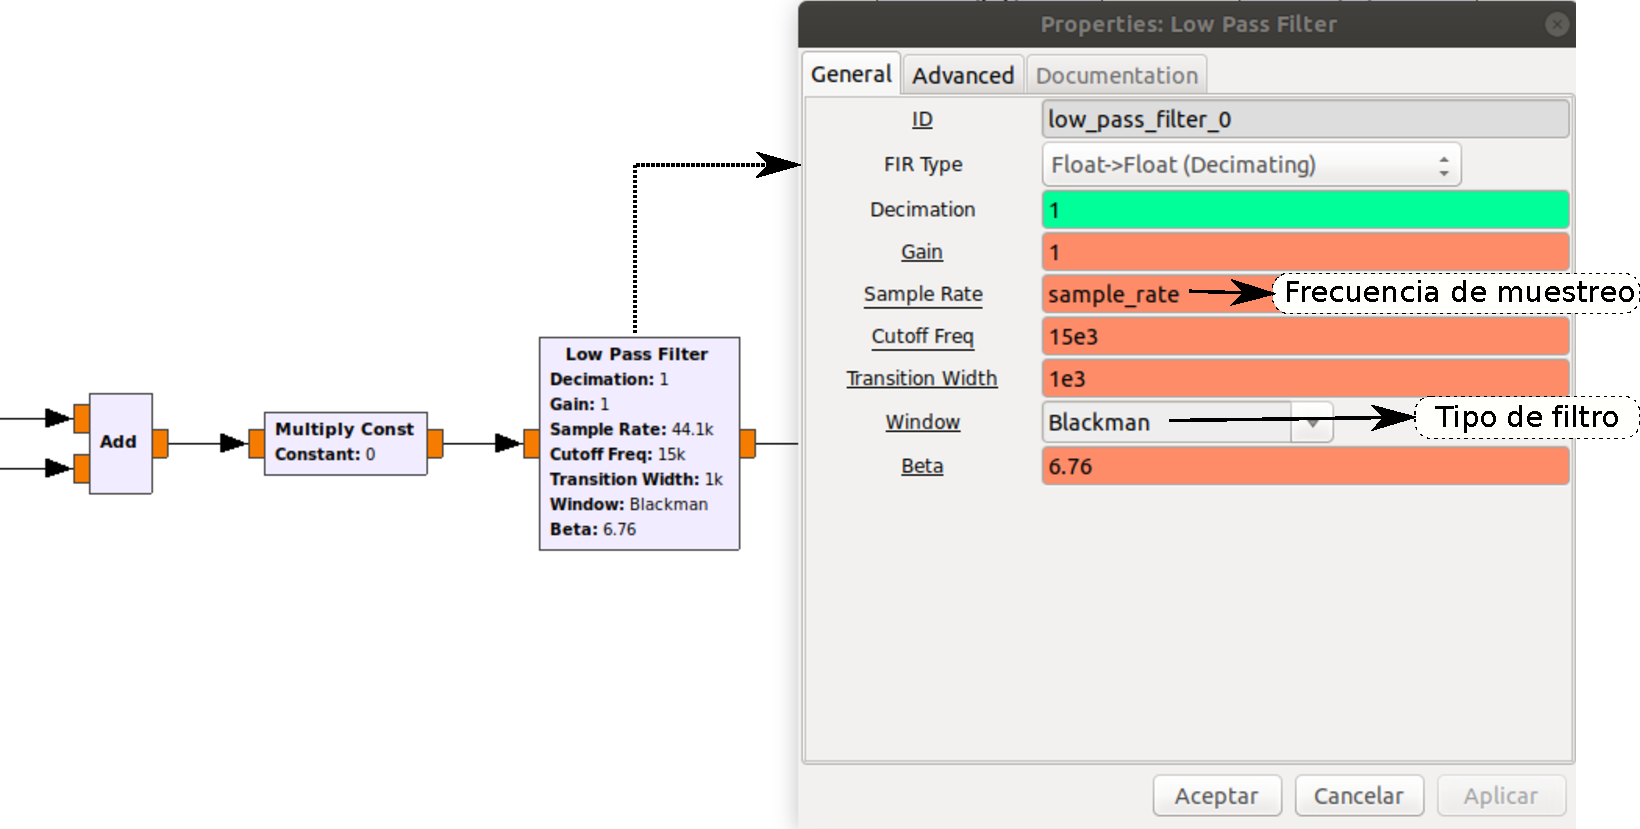
\includegraphics[width=\textwidth]{parte3/lab14/pdf/Lab14_5.pdf}
\end{figure}


\end{frame}
%---------------------------------

\begin{frame}{Desarrollo del diagrama en GNU Radio}

Ahora es necesario realizar la modulación de la señal en FM para ello se configuró el bloque WBFM Transmit.

\begin{figure}[H]
\centering
\vspace{-3mm}
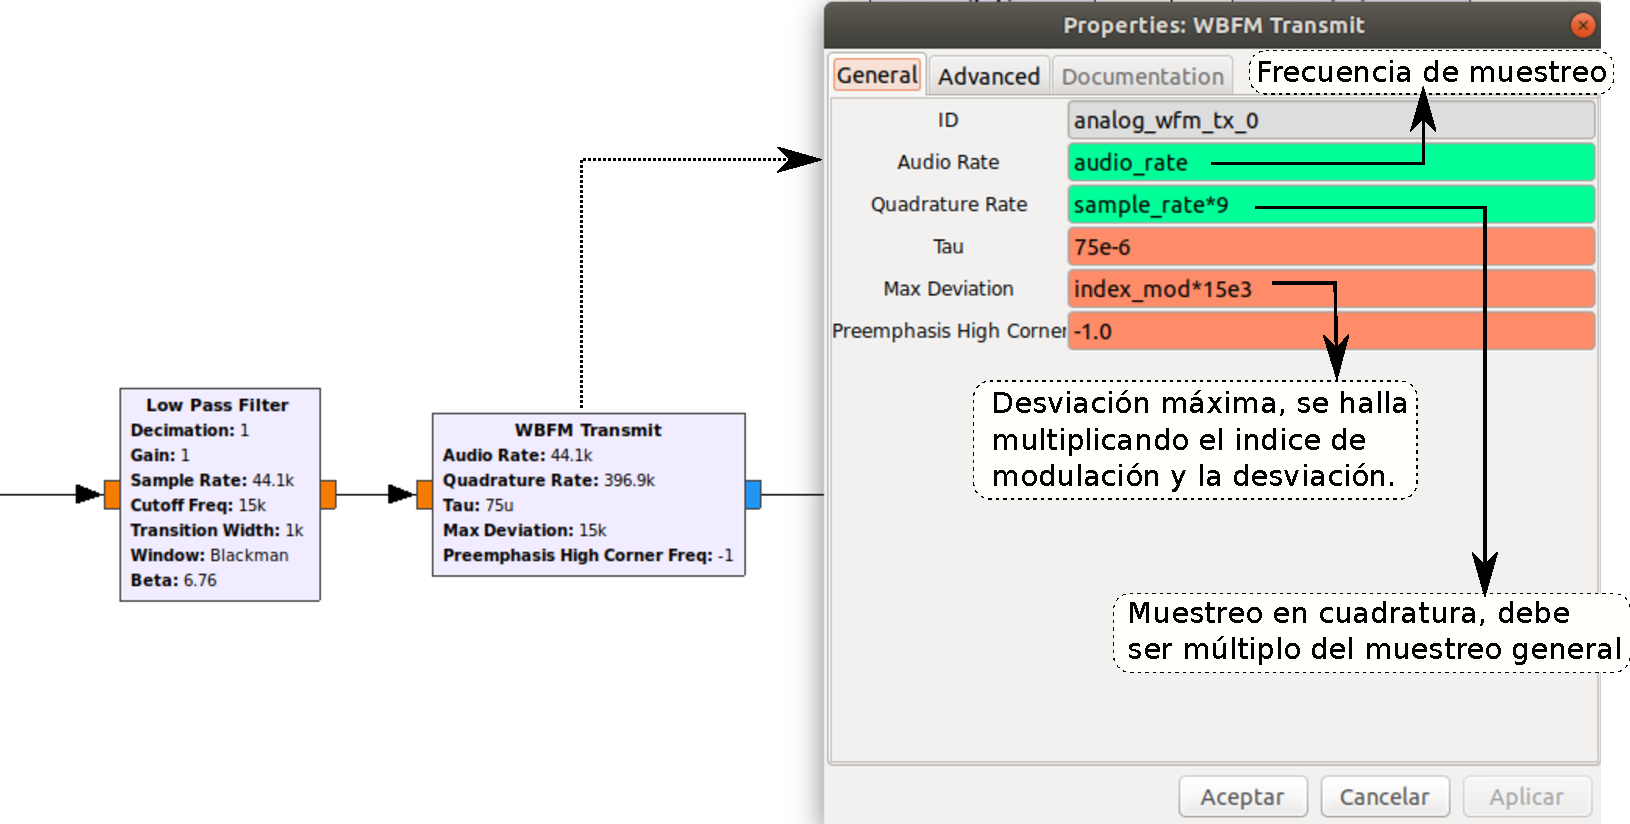
\includegraphics[width=\textwidth]{parte3/lab14/pdf/Lab14_6.pdf}
\end{figure}


\end{frame}
%---------------------------------

\begin{frame}{Desarrollo del diagrama en GNU Radio}

Antes de transmitir se realiza un re-muestreo a una frecuencia que permita a la tarjeta enviar el audio sin ningún problema.

\begin{figure}[H]
\centering
\vspace{-3mm}
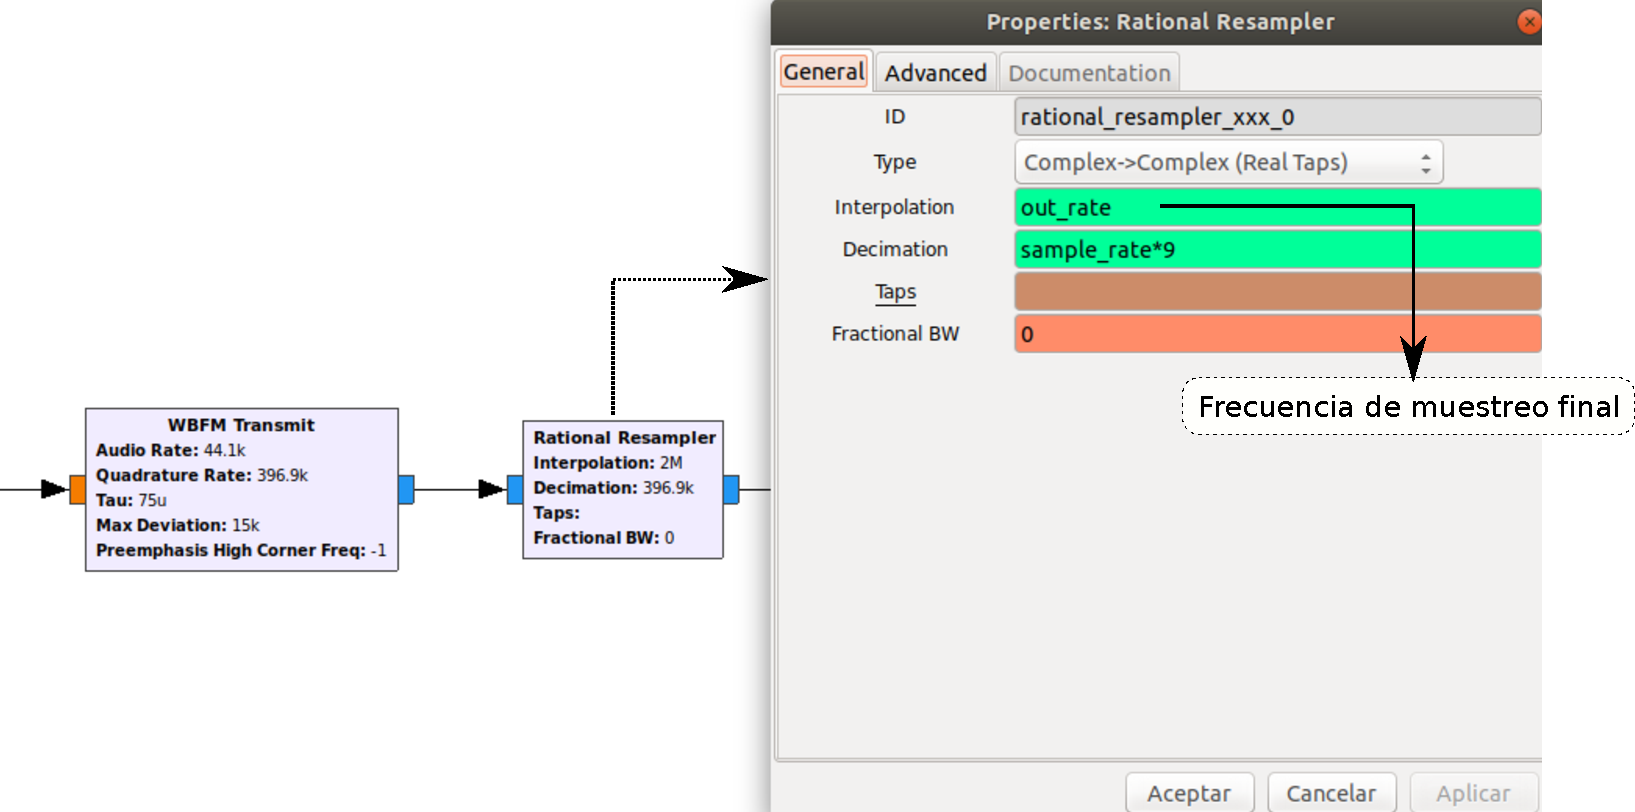
\includegraphics[width=\textwidth]{parte3/lab14/pdf/Lab14_7.pdf}
\end{figure}


\end{frame}
%---------------------------------

\begin{frame}{Desarrollo del diagrama en GNU Radio}

Finalmente se realiza la transmisión de la señal utilizando el bloque Osmocom Sink.

\begin{figure}[H]
\centering
\vspace{-3mm}
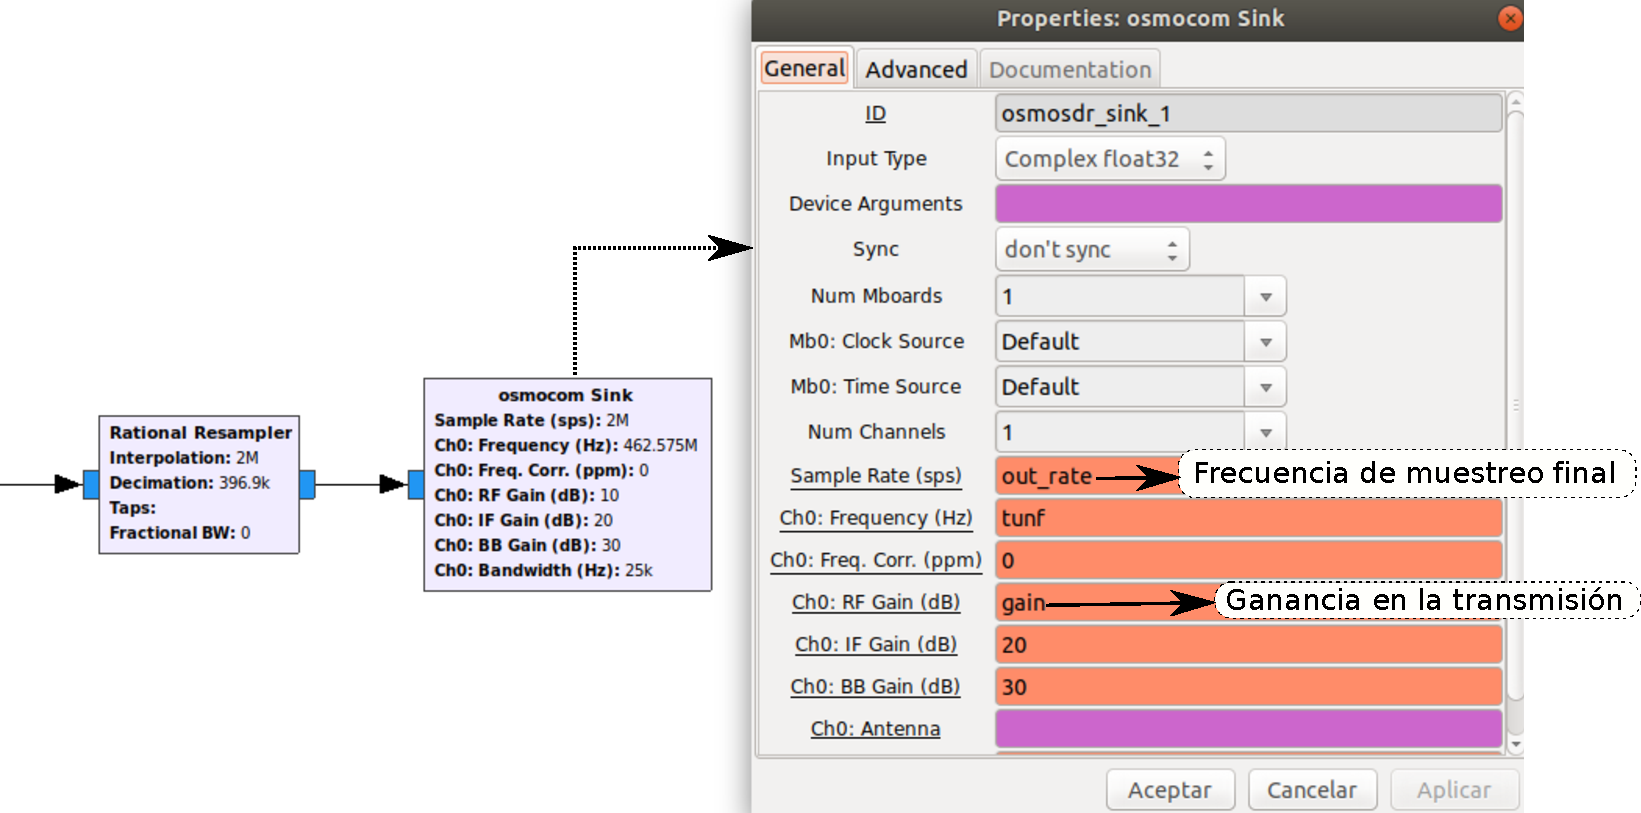
\includegraphics[width=\textwidth]{parte3/lab14/pdf/Lab14_8.pdf}
\end{figure}

\end{frame}
%---------------------------------

\begin{frame}{Interfaz gráfica}

La interfaz gráfica está compuesta por 3 páginas diferentes: la primera de ellas consiste en la transmisión final en términos de frecuencia, la segunda permite ver en la señal a transmitir en términos del tiempo y la tercera muestra la información entrante en términos de frecuencia como se puede observar a continuación:

\end{frame}
%---------------------------------

\begin{frame}{Interfaz gráfica}

\begin{figure}[H]
\centering
\vspace{-3mm}
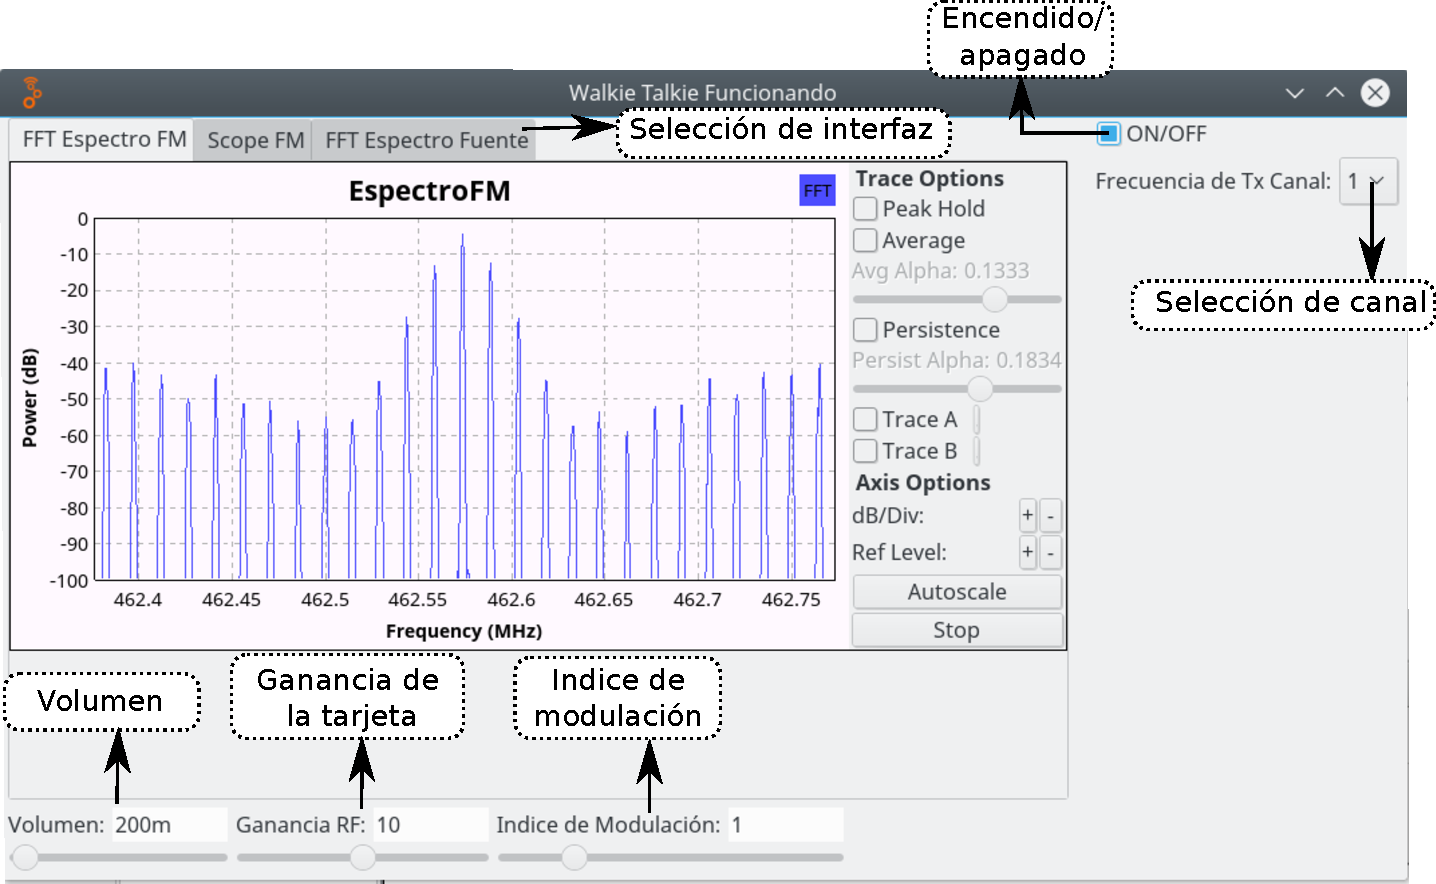
\includegraphics[width=0.9\textwidth]{parte3/lab14/pdf/Lab14_9.pdf}
\end{figure}

\end{frame}
%---------------------------------

\begin{frame}{Interfaz gráfica}

\begin{figure}[H]
\centering
\vspace{-3mm}
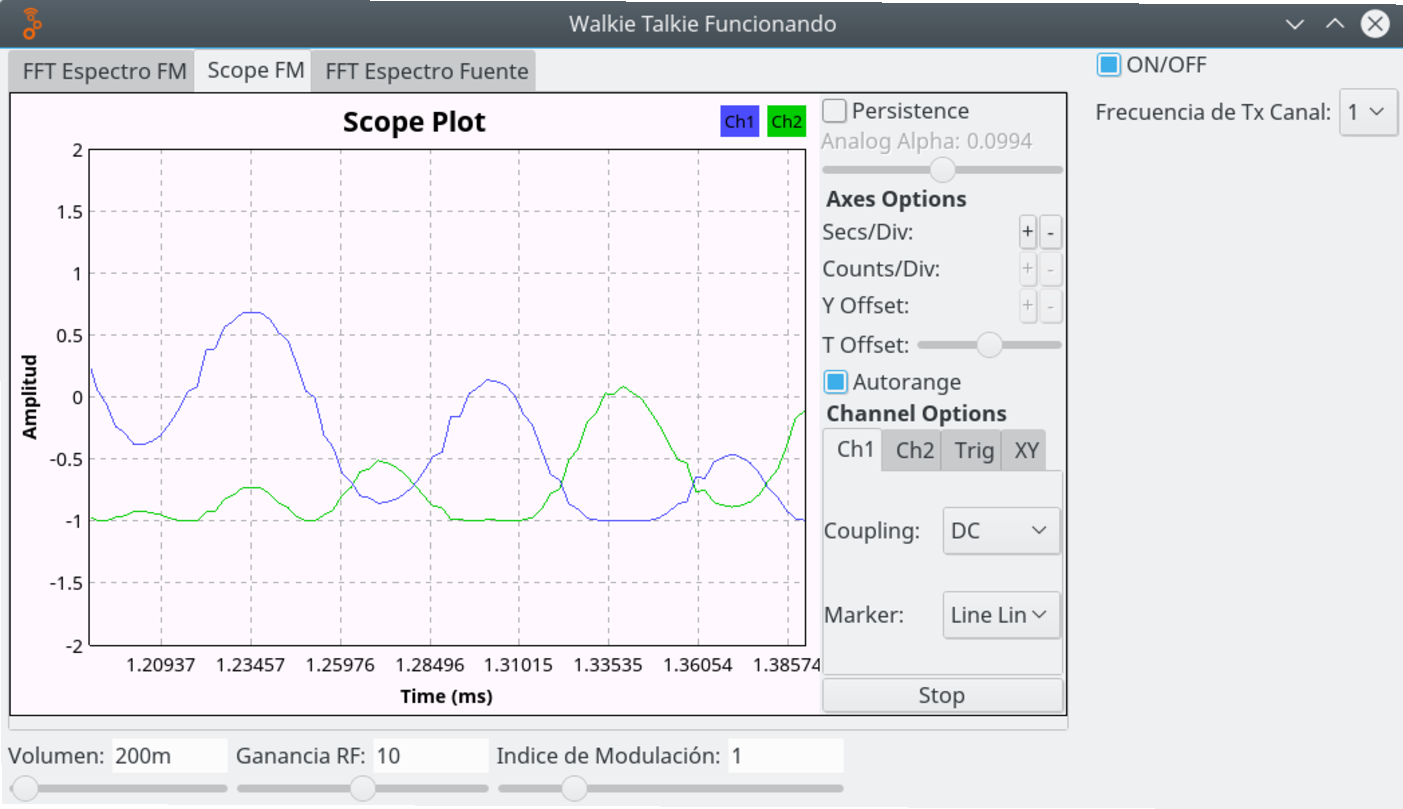
\includegraphics[width=0.9\textwidth]{parte3/lab14/pdf/Lab14_10.pdf}
\end{figure}

\end{frame}
%---------------------------------

\begin{frame}{Interfaz gráfica}

\begin{figure}[H]
\centering
\vspace{-3mm}
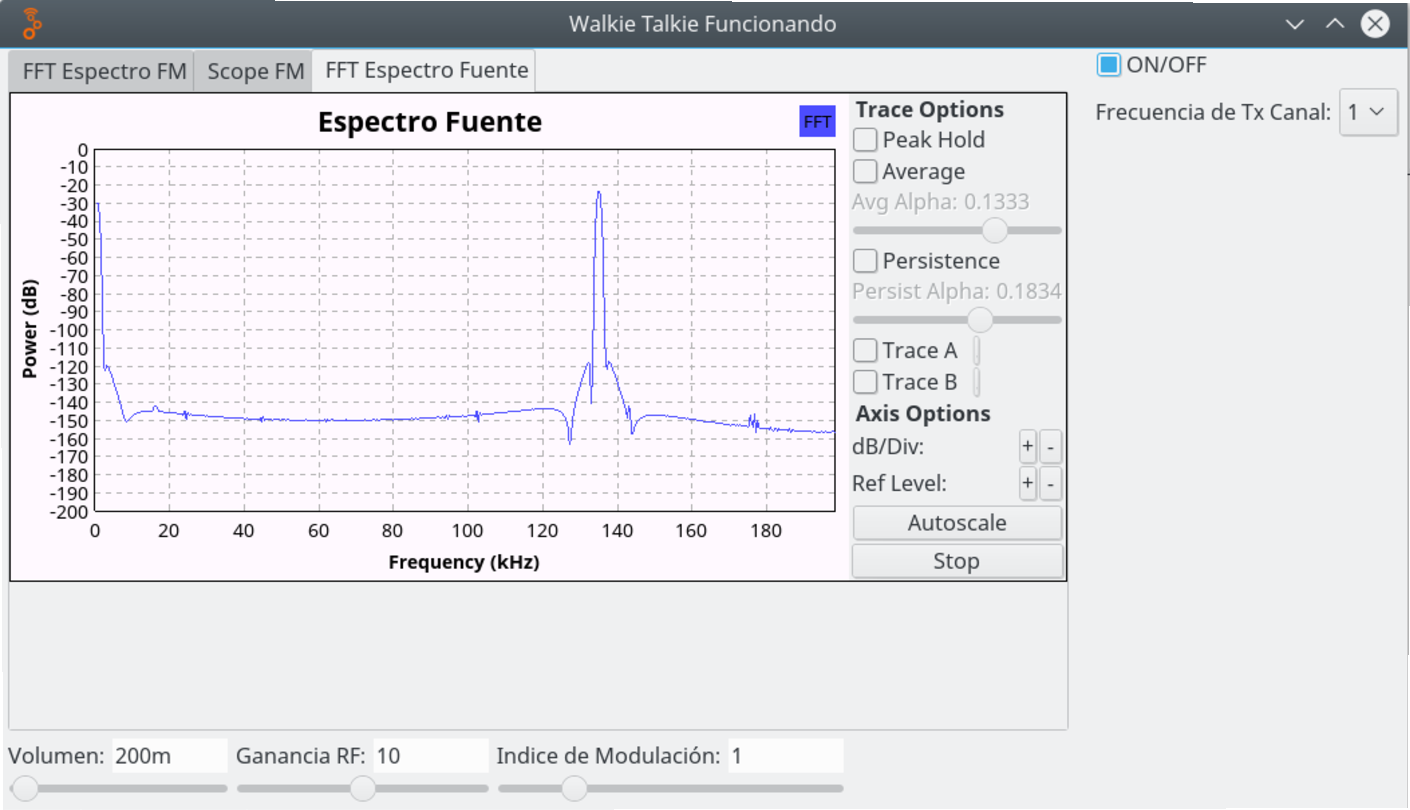
\includegraphics[width=0.9\textwidth]{parte3/lab14/pdf/Lab14_11.pdf}
\end{figure}

\end{frame}
%---------------------------------